\documentclass{beamer}
\mode<presentation>
% \usetheme{default}
% \usetheme{Boadilla}
% \usetheme{Madrid}
% \usetheme{Montpellier}
 \usetheme{Warsaw}
% \usetheme{Copenhagen}
% \usetheme{Goettingen}
% \usetheme{Hannover}
% \usetheme{Berkeley}
 
% \usecolortheme{crane}
 % \beamertemplatesolidbackgroundcolor{craneorange!25}
 
 \usepackage[utf8]{inputenc}
%\usepackage[T1]{fontenc}
\usepackage{amsmath,amssymb}
\usepackage[english,french]{babel}
%\usepackage{natbib}


\header{ \begin{center} 
\includegraphics[height=1.4cm]{ujf2.jpg} \end{center}}
 

\title[ED de Physique]{ED de Physique: parcours, recherche, thèse}




 
\author{Timothée Menais}
 
\institute[CEA] {\begin{center} 
\includegraphics[height=1.5cm]{cea.jpg} \hfill 
\includegraphics[height=1.2cm]{inac.jpg} \hfill

\includegraphics[height=1.4cm]{spram.jpg}\end{center}}


\setbeamertemplate{navigation symbols}{}


\begin{document}
\selectlanguage{french}

\frame[plain]{\titlepage} % # 1




\section{Parcours}
 
 
\frame % # 2
{
  \frametitle{Parcours}
 

\begin{itemize}
\begin{center}

\item<1-> Baccalauréat scientifique  

 Lycée Blaise Pascal, Longuenesse(62) (2006)
\medskip
\medskip


 \item<2-> Classe préparatoire	
 
 PCSI-PC* Lycée Henri Wallon, Valenciennes(59) (2006-2009)
 \medskip
\medskip
 
 \item<3-> ENS Lyon
 
 L3 et M1 Sciences de la matière (2009-2011)
 \medskip
\medskip

 \item<4-> INPG PHELMA
 
 M2R: EP Énergétique-Physique (2011-2012)
 \medskip
\medskip

Moyenne hors stage: 14.9 classement: 2/7

\end{center} 
\end{itemize}

}





 \frame % # 2
{
  \frametitle{Débuts académiques}

\begin{itemize}
\begin{center}

\item<1->  Ouverture à de nombreux domaines de la physique
\medskip
\item<2->  Physique statistique, méthodes numériques, matière molle 


\medskip
\medskip

\item<3-> Premières expériences de recherche grâce aux stages:
\medskip

\item<4-> \small{\mbox{L3: Reversibility and chaos: 3-body problem of sedimenting particles}

IUSTI: Marseille
}
\medskip


\item<4-> \small{\mbox{M1: Electrically driven transport of colloids in microuidic chips}

Cavendish Laboratory: Cambridge
}

\item<4-> \small{\mbox{M2: Theoretical study of biomolecules translocating through a nanopore}

INAC: CEA Grenoble
}


\end{center}
\end{itemize}

}

 
\section{Recherche récente}

\frame % 3
{
  \frametitle{Stage de M2}
  
   \begin{itemize}
  \begin{center}
  
 
\item<1-> Les nanopores ont de multiples applications:
  
  Médicales, biotechnologiques ...
  
  \medskip
  
\item<2-> Mais aussi un intérêt fondamental pour la physique statistique des polymères
  
\end{center}
\end{itemize}

\begin{columns}
\begin{column}{0.6\textwidth}

   \begin{itemize}
  \begin{center}
 \item<3-> Bio-pores:
 \medskip
 \medskip
 \medskip
 \medskip
 \medskip
 \medskip
 \medskip
 \medskip
 \medskip

 
 
 \item<4-> Pores artificiels:
  \end{center}
\end{itemize}

\end{column}
\begin{column}{0.6\textwidth}
\begin{center}
\uncover<3->{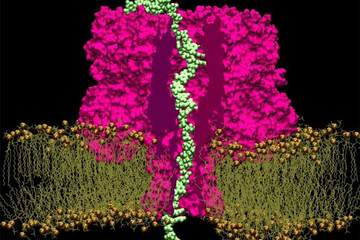
\includegraphics[width=0.45\textwidth]{biopore.jpg}}


\uncover<4->{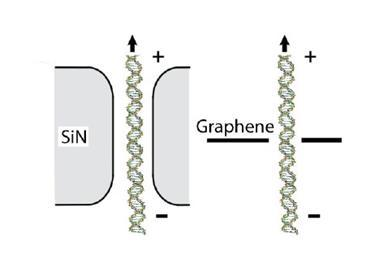
\includegraphics[width=0.55\textwidth]{nanopore.jpg}}
\end{center}
\end{column}
\end{columns}






}


 \frame % # 2
{
  \frametitle{Modèle utilisé}
   \begin{center}

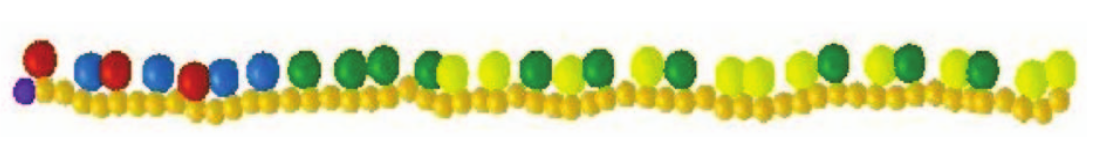
\includegraphics[width=0.9\textwidth]{screenmodel.png}

\medskip

\begin{columns}
 \begin{column}{0.6\textwidth}
\begin{itemize}
\item<2->{Modèle gros grains}
\medskip
\item<3->{Monocouche de carbones fixes}
\medskip
\item<4->{Potentiels d’intéractions}
\medskip
\medskip
\medskip
\medskip
\item<5->{Dynamique moléculaire}
\medskip
\item<6->{Comparaison physique statistique}


\end{itemize}
\end{column}
\begin{column}{0.4\textwidth}

\uncover<2->{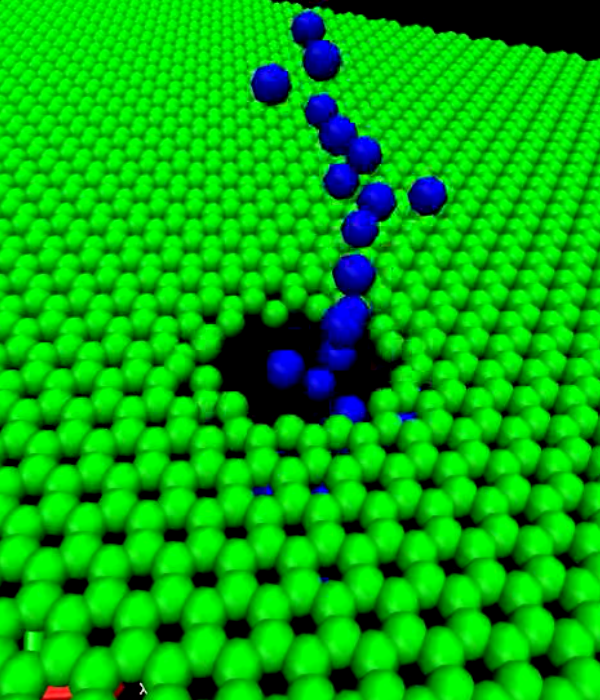
\includegraphics[width=\textwidth]{coarsegrain.png}}
\end{column}
\end{columns}
\end{center}

}


\frame
{
  \frametitle{Lois d'échelles}
  
  \begin{columns}
  \begin{column}{0.5\textwidth}
\begin{center}
Polymère libre

$D \sim N^{-1} $
\medskip

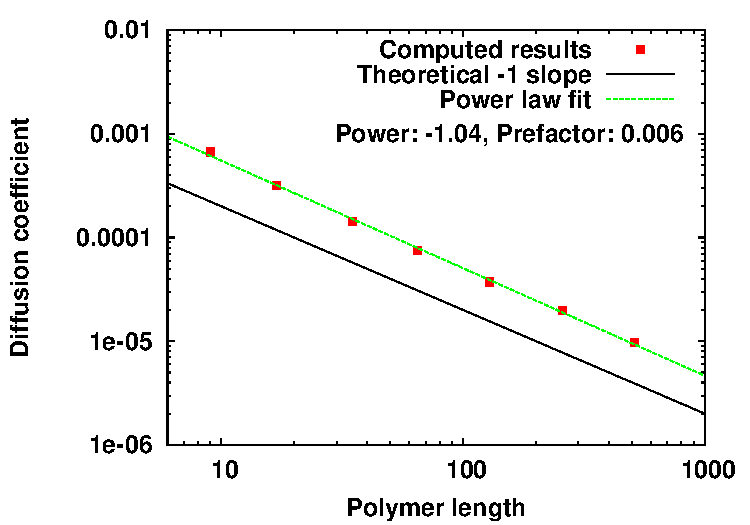
\includegraphics[width=1.15\textwidth]{diffusioncoefficient.pdf}
\end{center}

\end{column}

\begin{column}{0.5\textwidth}
  
\begin{center}
Translocation

$\tau \sim N^{1.73} $
\medskip


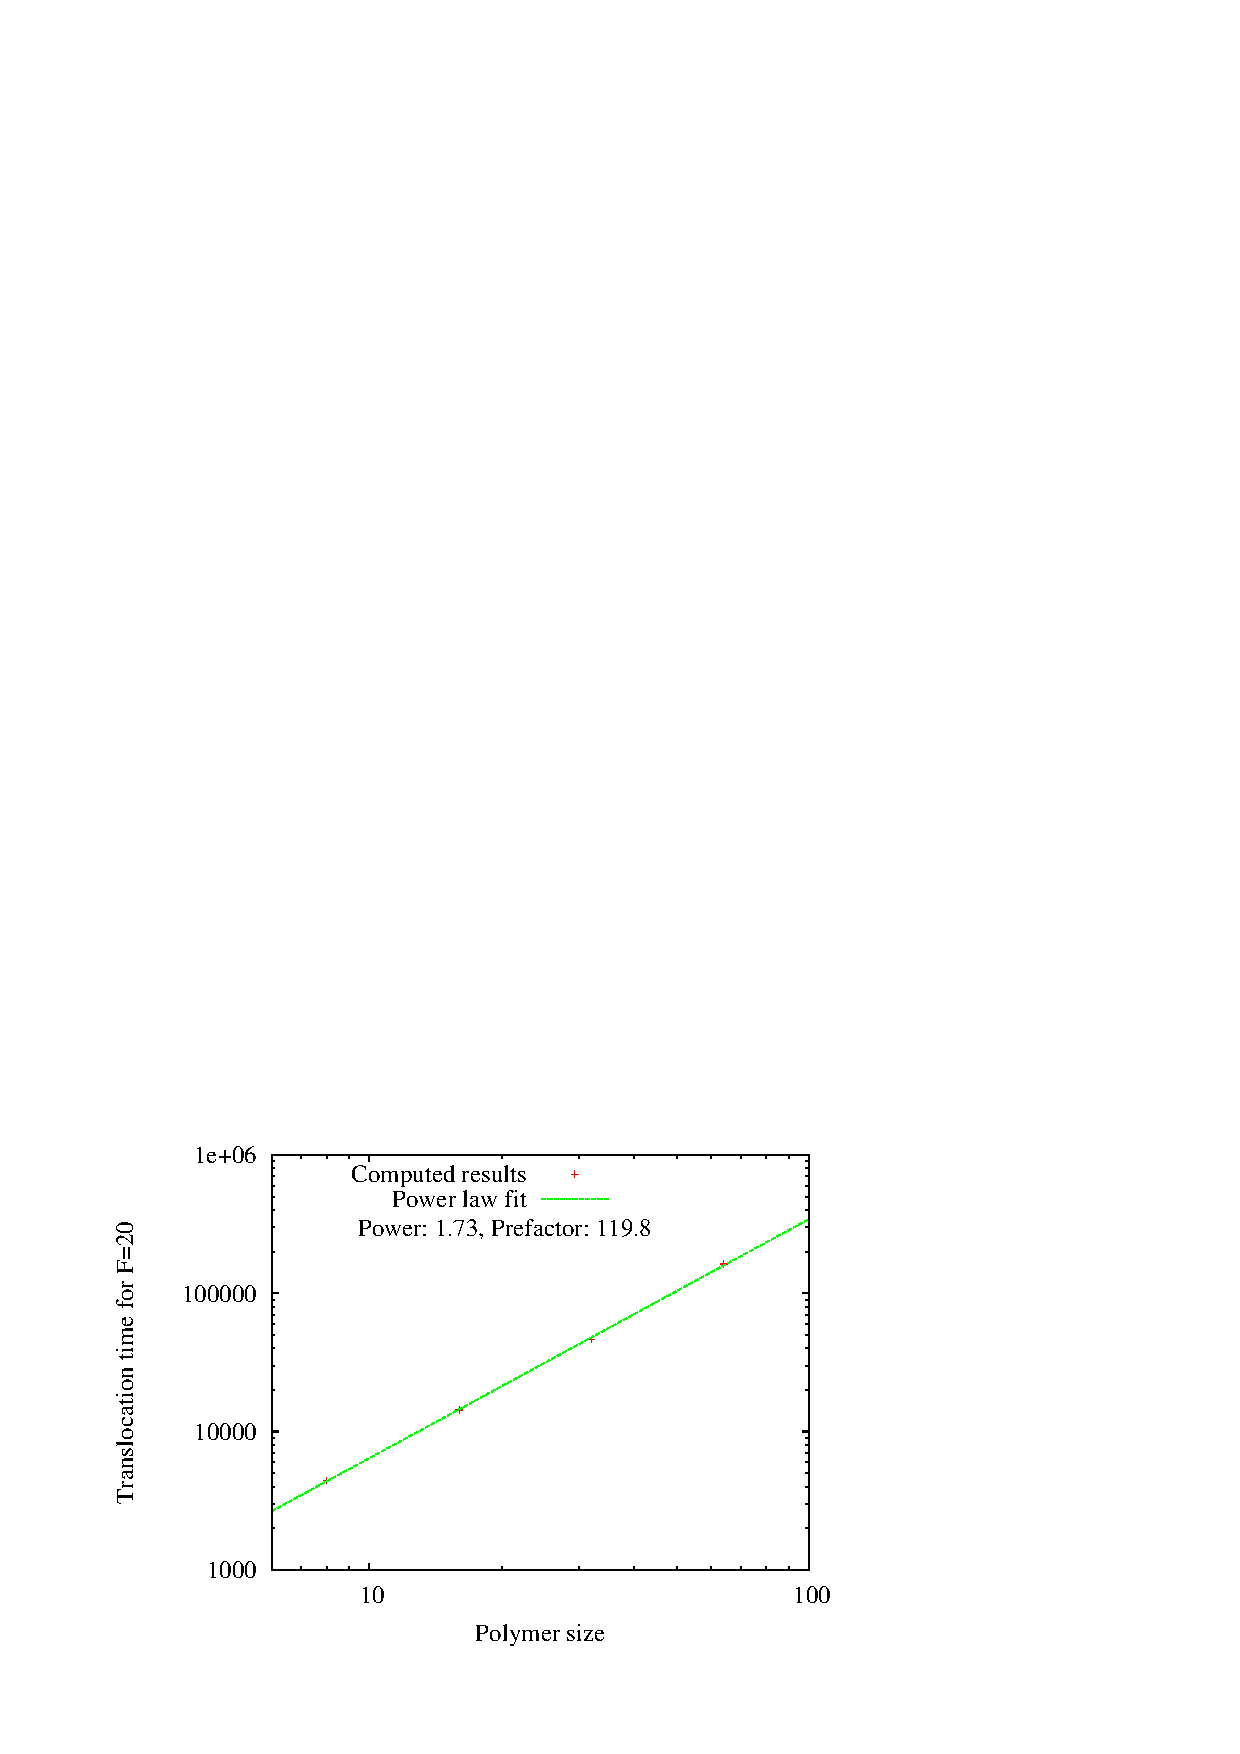
\includegraphics[width=1.15\textwidth]{tauxf20.pdf}
\end{center}
\end{column}
\end{columns}
}

\section{Poursuite en thèse}
\frame % # 2
{
  \frametitle{Encadrement de la thèse}
 
 \begin{center}
 
\includegraphics[height=1.5cm]{cea.jpg} \hfill 
\includegraphics[height=1.2cm]{inac.jpg} \hfill

\includegraphics[height=1.4cm]{spram.jpg}
 \end{center}

\begin{itemize}
\begin{center}

\item<1-> Arnaud Buhot
\item<2-> Stefano Mossa

\medskip

\item<3-> Compétences en méthodes numériques et physique statistique

\medskip
\item<4-> Ressources numériques disponibles (Clusters de calculs)


\end{center}
\end{itemize}
}




\frame % # 2
{
  \frametitle{Sujet de thèse}
 
\begin{itemize}
\begin{center}

\item<1-> \mbox{Utiliser les bases acquises pour aborder de nouvelles problématiques}
\medskip
\item<2-> Accent sur les vibrations et la flexibilité particulières au graphène
\uncover<2->{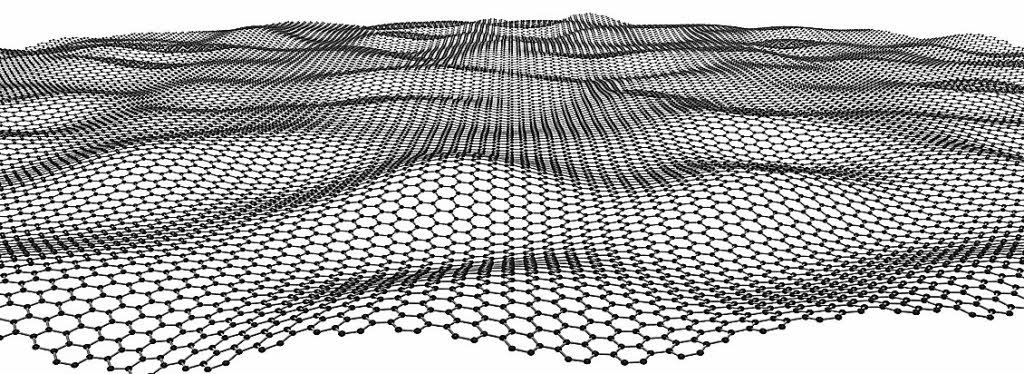
\includegraphics[width=0.9\textwidth]{vib.jpg}}
\medskip

\item<3-> Calculs numériques et modélisation analytique
\medskip
\medskip

 \end{center}
\end{itemize}


}

\frame % # 2
{
  \frametitle{Perspectives}
 

\begin{itemize}
\begin{center}

\item<1-> Thèse: point de départ pour une carrière académique  
\medskip
\item<2-> Intérêt scientifique
\medskip
\item<3-> Possibilité d'enseigner
\medskip
\item<4-> Étape logique pour devenir enseignant chercheur
\medskip

 \end{center}
\end{itemize}

}


\frame % 3
{
  \frametitle{Conclusion}
 
 
 
 
 \begin{center}
 {\HUGE Merci de votre attention.
 
 
 \pause
 \medskip
 Des questions ?}
 \end{center}
 
 


}

\frame
{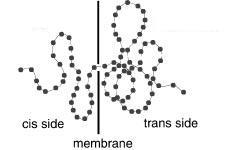
\includegraphics[width=0.9\textwidth]{transloc.pdf}
}



\end{document}
       
 